\documentclass[11pt]{article}

\renewcommand{\familydefault}{\sfdefault}

% Make margins smaller
\usepackage[top=1.1in, bottom=1.1in, left=1.1in, right=1.1in]{geometry}
% more advanced mathematical symbols
\usepackage{amsfonts}
\usepackage{amssymb}
\usepackage{amsmath}
\usepackage{bm}
\usepackage{bold-extra} % bold texttt
\usepackage{graphicx}
\usepackage{enumerate}
\usepackage[font=small,labelfont=bf]{caption} % Required for specifying captions to tables and figures
\usepackage{pgfgantt} % gantt chart!
\usepackage{setspace}
\renewcommand{\baselinestretch}{1.2}

\graphicspath{ {./images/} }

\begin{document}

\title{\textbf{Machine Learning Summative}}
\date{for 22nd March 2019}
\author{wbbz74}
\maketitle 

\section{Image Classifier}

% MAYBE DON'T TREAT IT SO MUCH AS A NARATIVE AND DON'T SHOW SO MANY GRAPHS OF THE PERFORMANCE? JUST TALK ABOUT SPECIFIC THINGS THAT DID/DIDN'T WORK

\subsection{Linear Network}

The base network consists of a simple, 3 layer fully connected network containing only 1 hidden layer. This performs poorly as there is little opportunity for the network to learn deep and abstract representations by using a single hidden layer. Additionally, spatially related information is not considered together---a vital aspect of an image classification task, where neighbouring pixels need to be considered as a unit in order to identify items in given images. 

It was quickly established that the greater number of epochs, the greater overall accuracy of the trained network. After around 50 epochs, this network only shows accuracy of around 15\%, also showing signs of overfitting as the training data starts to obtain higher recall accurately than the test data.

    \begin{center}
        \begin{minipage}{0.75\linewidth}
            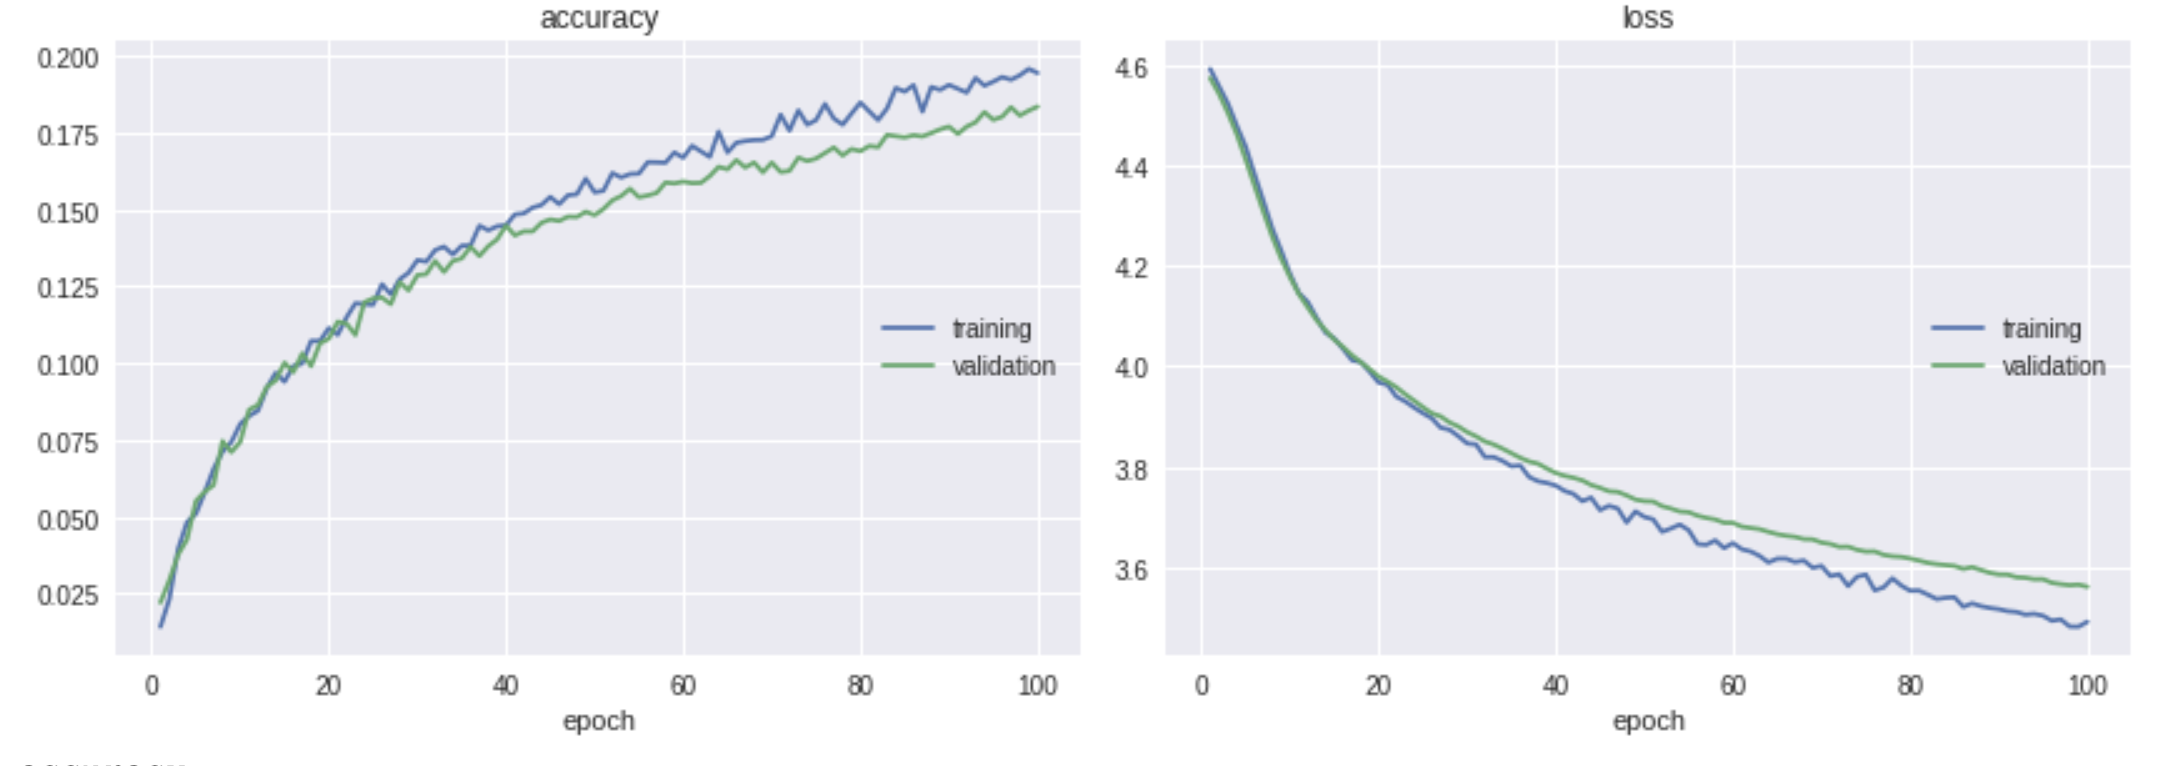
\includegraphics[width=\linewidth]{accuracy0}
            \captionof{figure}{Initial accuracy, 3 fully connected layers (1 hidden) with ReLU normalisation.}
        \end{minipage}%
    \end{center}
    
\subsection{Convolutional Networks}

To remedy this, we replace the pure linear structure of the network with a convolution based network. Convolutional Neural Networks (CNNs) are able to better learn representations based on a number of spatially related inputs, allowing for better generalisation of image data. This is achieved by learning convolution masks and which reduce the dimensionality of the image. We would expect to see vastly improved performance adopting a convolutional based network.

My first modified network consisted of 2 convolutional layers, each followed by a max pooling layer (2x2). Then, flattening this output, it is passed to two hidden fully-connected layers before the final classification layer. As shown in Figure \ref{fig:first-conv}, after 100 epochs the network shows far fewer signs of overfitting as the accuracy climbs past 20\%. However, the accuracy did not climb as quickly as I expected it to compared to the prior network.

\begin{small}
\begin{verbatim}
class BetterNetwork(nn.Module):

    def __init__(self):
        super(BetterNetwork, self).__init__()
        self.conv = nn.Sequential(
            nn.Conv2d(3,6,5),
            nn.MaxPool2d(2,2),
            nn.ReLU(),
            nn.Conv2d(6,12,3),
            nn.MaxPool2d(2,2),
            nn.ReLU()
        )
        self.lin = nn.Sequential(
            nn.Linear(in_features=432, out_features=512),
            nn.ReLU(),
            nn.Linear(in_features=512, out_features=100)
        )

    def forward(self, x):
        for l in self.conv:
            x = l(x)
        x = x.view(x.size(0), -1) # flatten
        for l in self.lin:
            x = l(x)
        return x
\end{verbatim}
\end{small}


    \begin{center}
        \begin{minipage}{0.75\linewidth}
            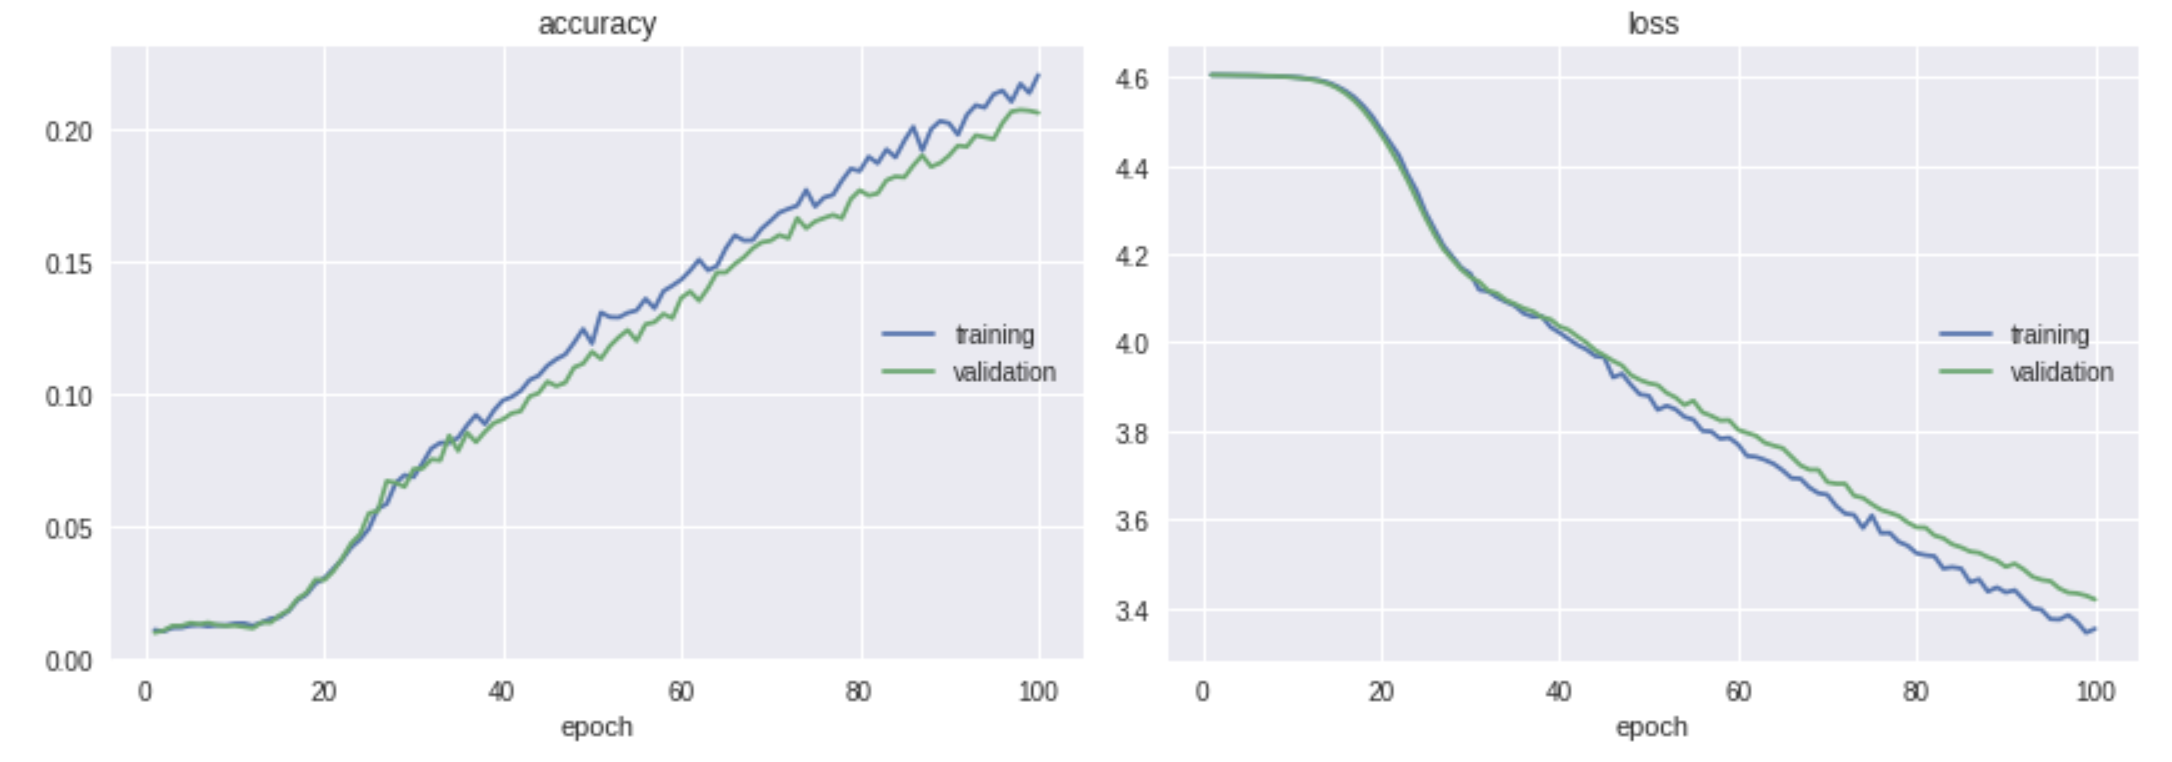
\includegraphics[width=\linewidth]{accuracy1}
            \captionof{figure}{Initial convolution based network (2 conv2d layers, 2 maxpooling, 2 fully-connected layers.}
            \label{fig:first-conv}
        \end{minipage}%
    \end{center}
    
\subsection{Regularisation \& Optimiser}

To reduce the signs of this overfitting and to train a more accurate network, I added dropout layers after each max pooling and the first fully connected layer, each with probability 0.1. We clearly notice far similar performance for training and validation, such that allowing the training to run for around 180 epochs yields a far better network, with overfitting starting to occur much later. 

    \begin{center}
        \begin{minipage}{0.75\linewidth}
            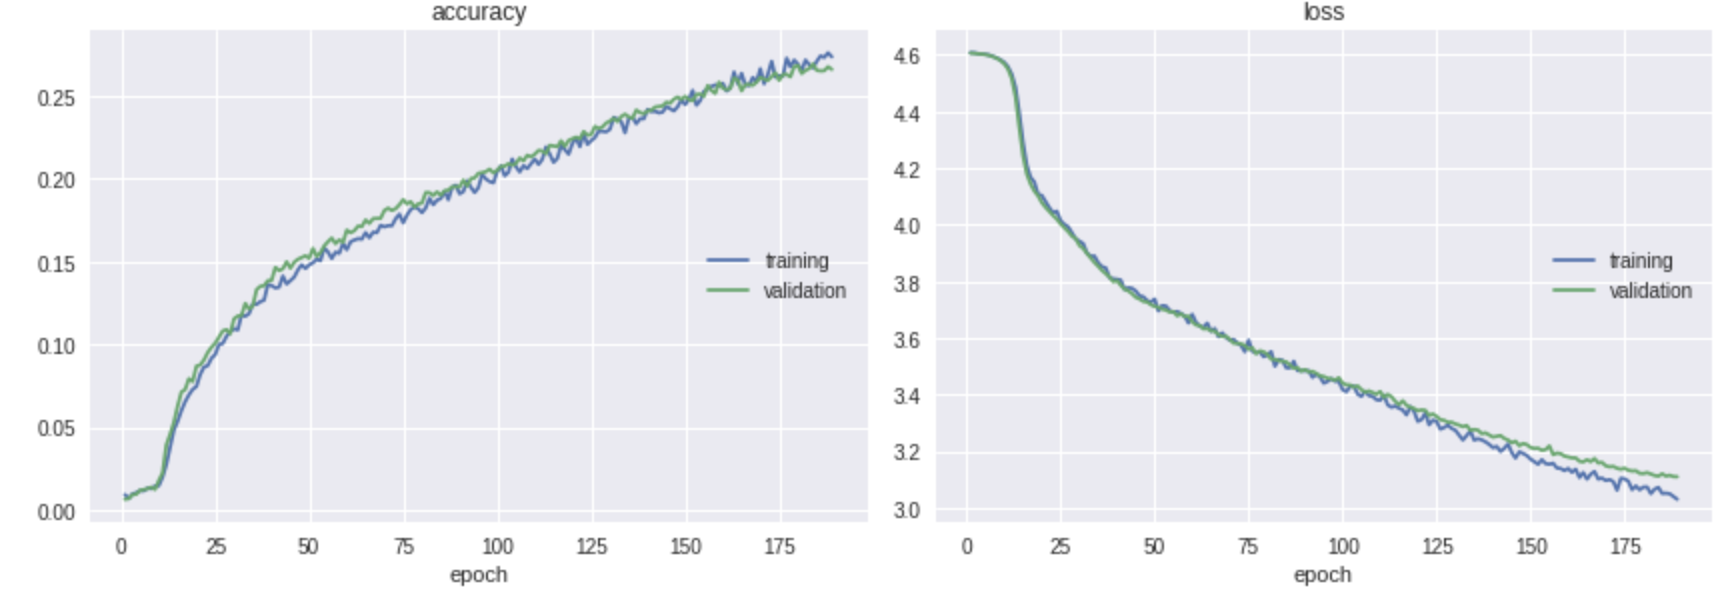
\includegraphics[width=\linewidth]{accuracy2}
            \captionof{figure}{Dropout layers (p=0.2) after each network segment.}
            \label{fig:first-conv}
        \end{minipage}%
    \end{center}

Changing this dropout later to 0.2, I noticed marginal improvements to this point where the overtraining occurs.

The most remarkable improvement occurred when changing the optimiser to \textit{Adam}. The network learned far more quickly, but also began overfitting far more quickly after only around 10 epochs. This, however, is still a vast improvement.


    \begin{center}
        \begin{minipage}{0.75\linewidth}
            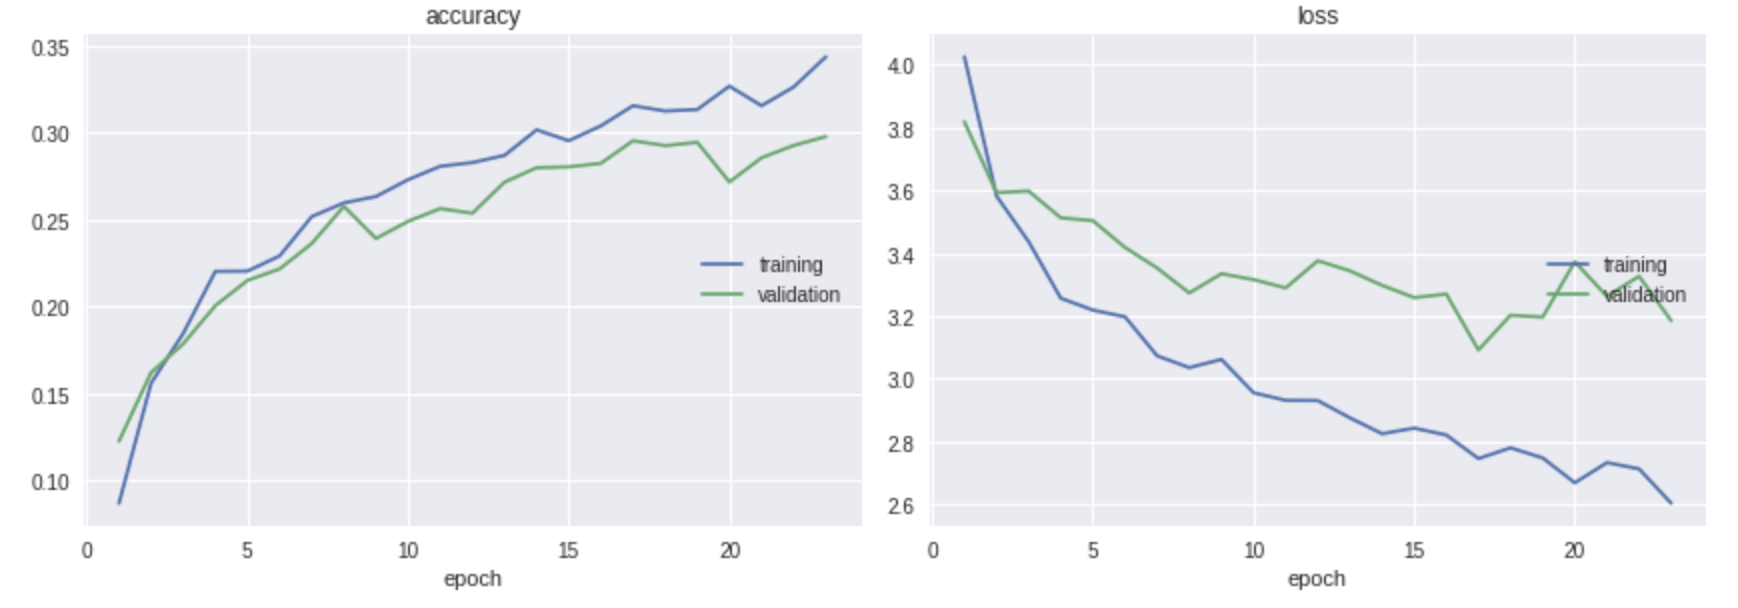
\includegraphics[width=\linewidth]{accuracy3}
            \captionof{figure}{Adam optimiser. Learns---and overfits---far more quickly.}
            \label{fig:first-conv}
        \end{minipage}%
    \end{center}
    
This overfitting was able to be slightly reduced by making improvements to the core network. Namely, using smaller convolution kernels of \texttt{3x3} for each convolutional layer and reducing the output channel sizes to 5 and 8 (from 6 and 12). A small improvement is able to be observed.

   \begin{center}
        \begin{minipage}{0.75\linewidth}
            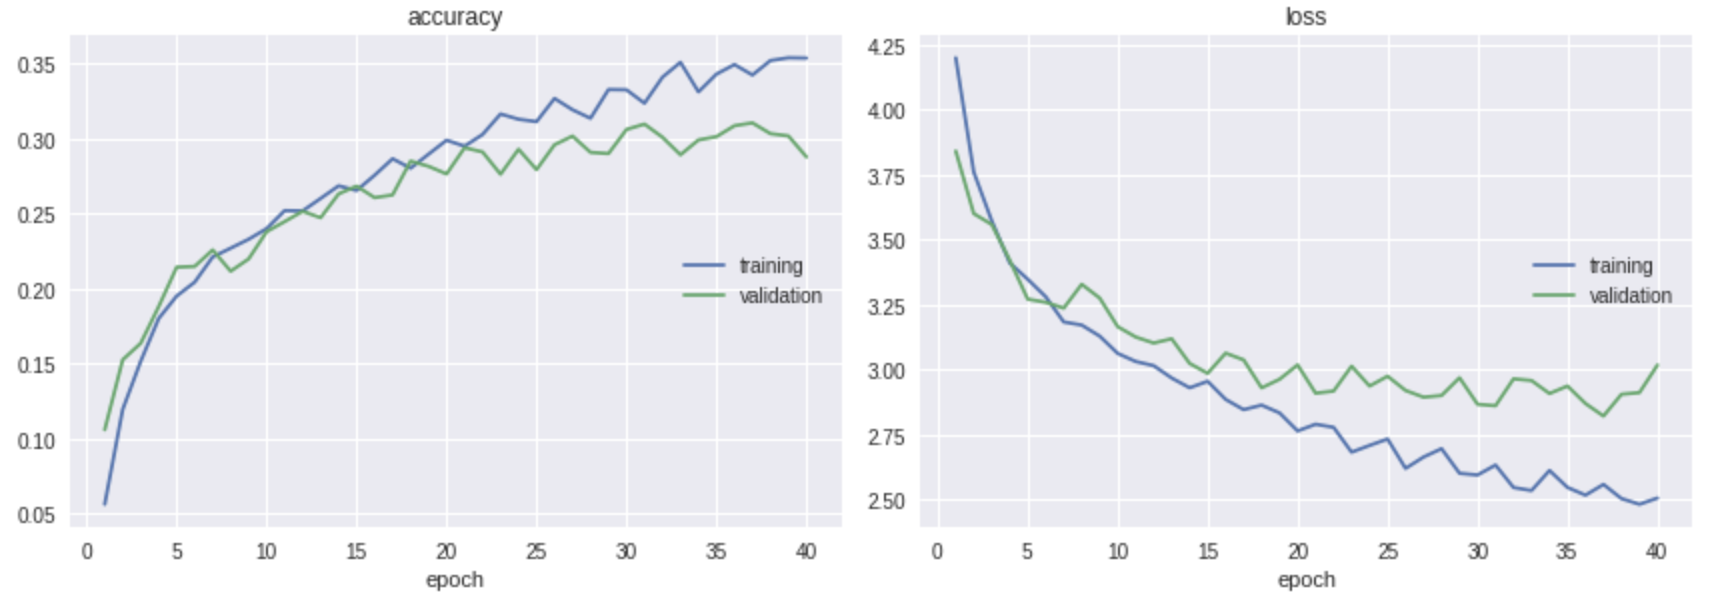
\includegraphics[width=\linewidth]{accuracy4}
            \captionof{figure}{After modification---slightly reduced overfitting.}
            \label{fig:first-conv}
        \end{minipage}%
    \end{center}
    
I found that augmenting the training images with random rotations, saturation changes and flips reduced the effect of the overfitting on the network and was able to achieve roughly the same peak accuracy on the test set of around 30\%, but took far longer to train (25 vs. 115 epochs until overfitting). In further tests, I found it prevented optimal accuracy of the network on the test dataset, so I disabled this. This is likely due to relatively small size of the network not being able to account well for these adaptations; a much deeper network with possibly a larger training set may have allowed these adaptations to increase recall performance.

   \begin{center}
        \begin{minipage}{0.75\linewidth}
            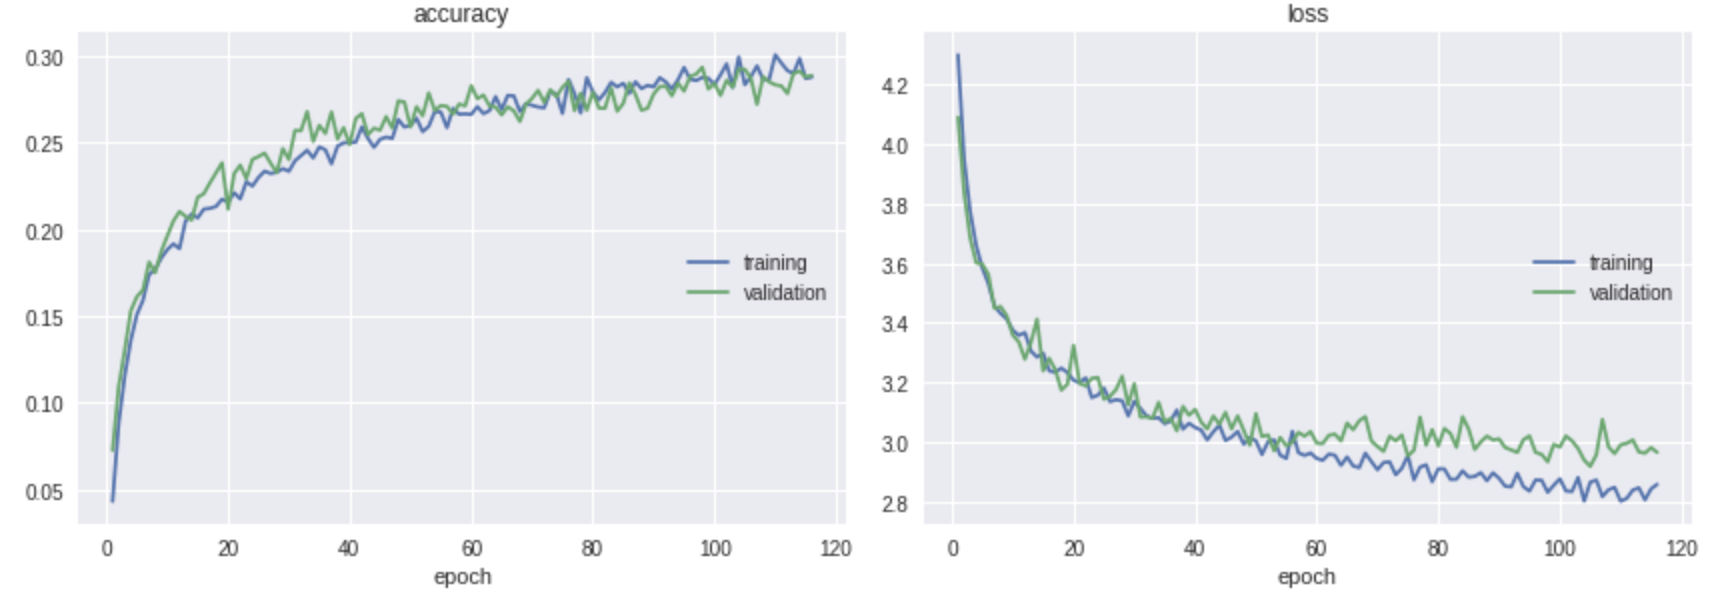
\includegraphics[width=\linewidth]{accuracy5}
            \captionof{figure}{Far longer training with image augmentation, obtaining similar peak accuracy of around 30\%.}
            \label{fig:first-conv}
        \end{minipage}%
    \end{center}
    
Additionally, I found that batch normalisation on the output of the convolutional layers was able to further increase the amount of time before over-fitting occurs and offered a slight increase in the accuracy of the network.

\subsection{Further Network Improvements}

% place for additional things to push the network to be the best it can possibly be

After experimenting with tweaks to the dimensions of the penultimate linear layer I found that size had little effect (unless made to be far too small ($<30$) or far too large ($>2048$) where performance slightly reduced) on network performance. Additionally, I found adding more than 3 hidden linear layers resulted in reduced network accuracy after a similar number of epochs and the network struggles to improve, also increasing the likelihood of overfitting. This occurred for a variety of sizes.

    \begin{center}
        \begin{minipage}{0.75\linewidth}
            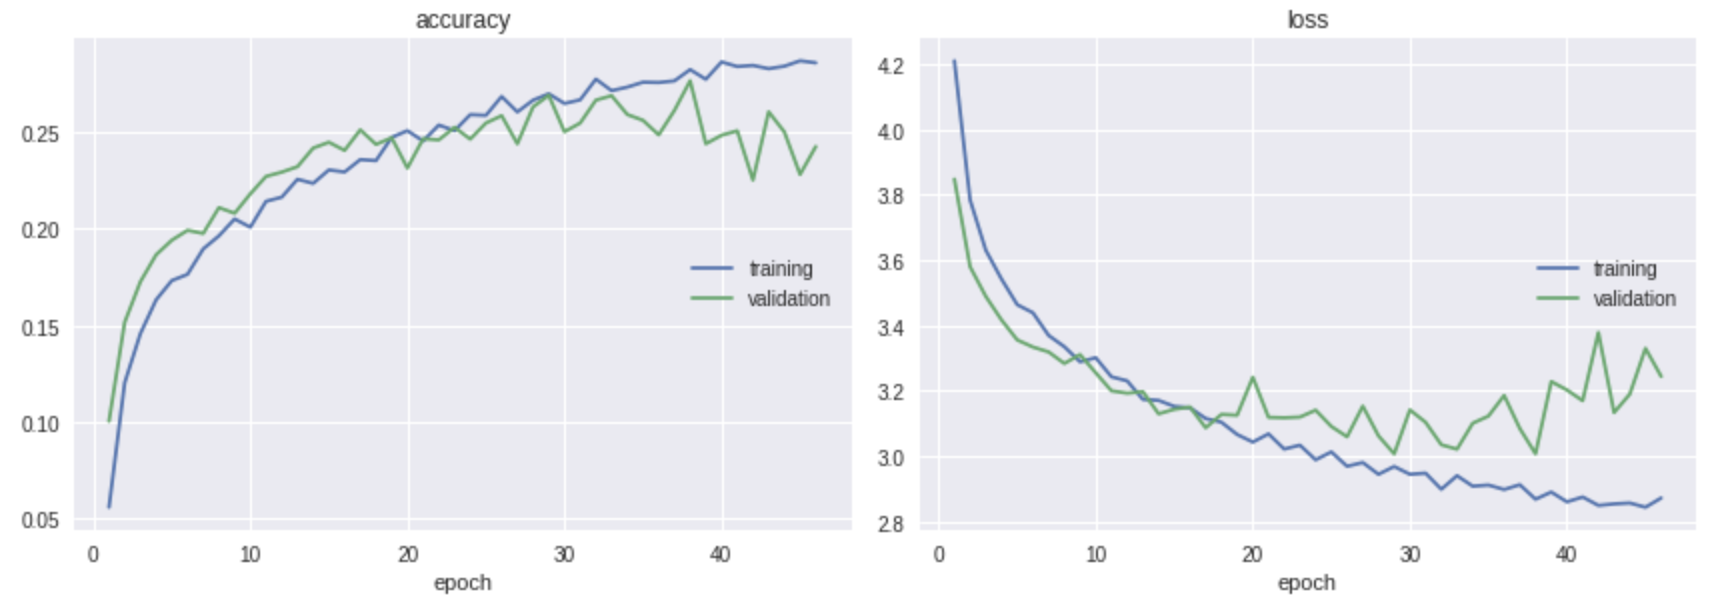
\includegraphics[width=\linewidth]{accuracy6}
            \captionof{figure}{4 hidden linear layers, greater likelihood of overfitting later on.}
        \end{minipage}%
    \end{center}
    
Next, I increased the batch size to 32. This should better inform the network at each step how to adjust the particular weights, as more of the dataset is considered at each learning step. I then added another convolution to the network and dramatically increased the number of channels output by each:

\begin{small}
\begin{verbatim}
self.conv = nn.Sequential(
    nn.Conv2d(3,16,3,stride=2),
    nn.Dropout(0.2),
    nn.BatchNorm2d(16),
    nn.ReLU(),
    nn.Conv2d(16,32,3,stride=2),
    nn.Dropout(0.1),
    nn.BatchNorm2d(32),
    nn.ReLU(),
    nn.Conv2d(32,32,3,stride=2),
    nn.Dropout(0.1),
    nn.ReLU()
)
self.lin = nn.Sequential(
    nn.Linear(in_features=288, out_features=512),
    nn.ReLU(),
    nn.Linear(in_features=512, out_features=100)
)
\end{verbatim}
\end{small}

This allowed for much less overfitting and the network to confidently achieve classification accuracy of around 35\%.

     \begin{center} % 0.348 accuracy
        \begin{minipage}{0.75\linewidth}
            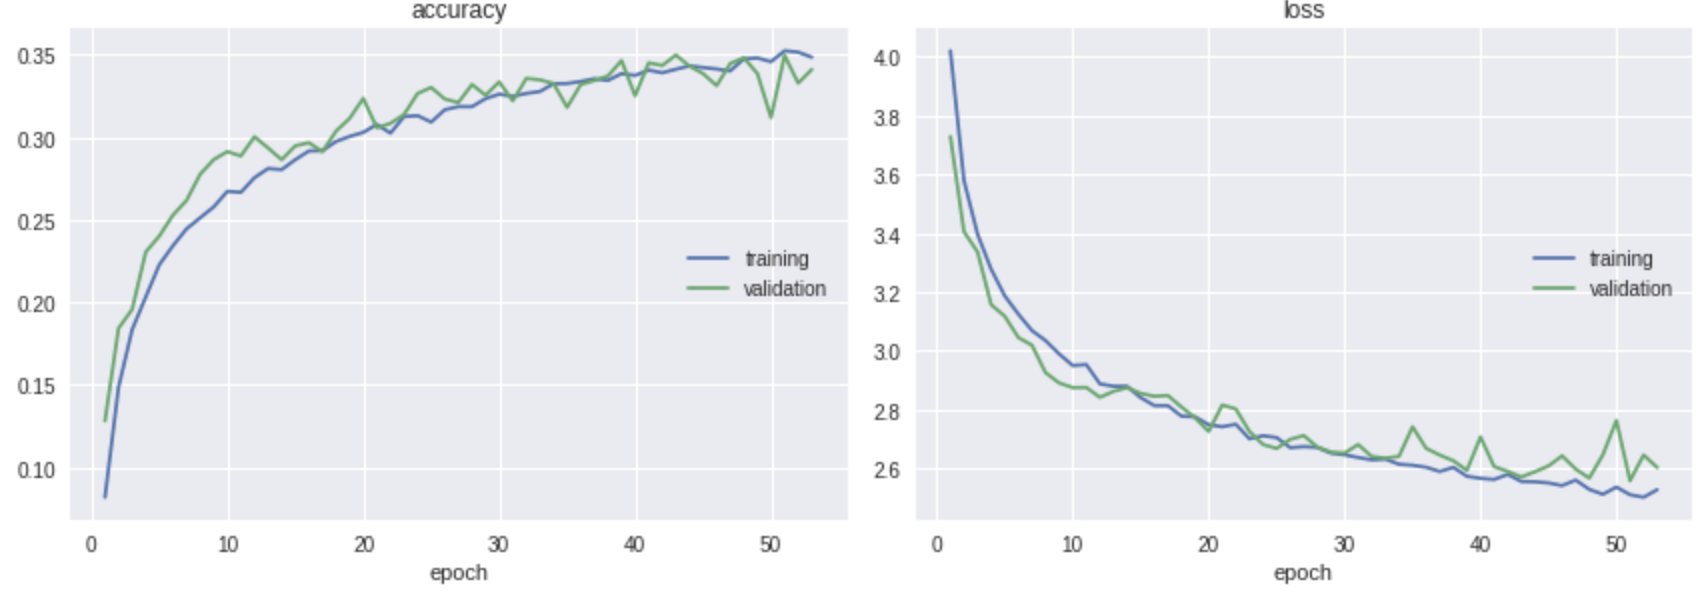
\includegraphics[width=\linewidth]{accuracy7}
            \captionof{figure}{Updated network, featuring much larger output channels from convolutions.}
        \end{minipage}%
    \end{center}
    

For my final network, I decided to test the effect of having a very large number of channels output by the convolutional networks. I adjusted the convolutional layers to increase rapidly to 64 channels, also adding 2 layers. Additionally, another linear layer was added. This was to allow the network more opportunities to learn deep representations.  This network performed better; training was terminated after around 50 epochs, when overfitting became clearly evident. The best test accuracy I was able to obtain is \textbf{42.1\%}.

     \begin{center} % 0.348 accuracy
        \begin{minipage}{0.75\linewidth}
            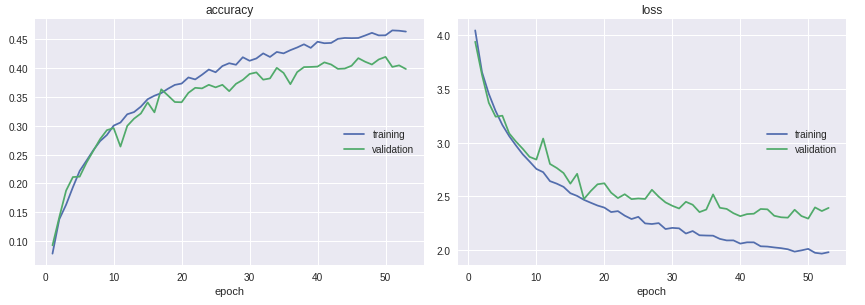
\includegraphics[width=\linewidth]{accuracy10}
            \captionof{figure}{The final network, consisting of 5 convolutional and 3 linear layers.}
        \end{minipage}%
    \end{center}

\section{Generating a Pegasus}

In order to achieve the best possible looking pegasus, we use a GAN at the core of the network, which has been able to achieve state of the art results in recent image generation tasks.


\end{document}